\section{Results}
We describe the results of our experiments with the three datasets. Section 2.4.1 compares between four learning methods and several baselines. It identifies the best metric-learning method for further analysis. Based on this method, section 2.4.2 identifies perceptually-discriminative features from the datasets in English. Finally, section 2.4.3 examines differences between the resulting metrics for Hebrew and English.

\subsection{Metric learning for phonemes}
We compare four methods for learning an optimal metric function: LS, diagonal-LS, OASIS, diagonal-OASIS, and compare them to three baseline methods - uniform weights, PMV and Frisch-similarity (sections 2.2.2, 2.2.3). To single out the best method we evaluate the predictive power of the metric function of each method.

\begin{figure}[H]
\vspace{.3in}
\makebox[\textwidth][c]{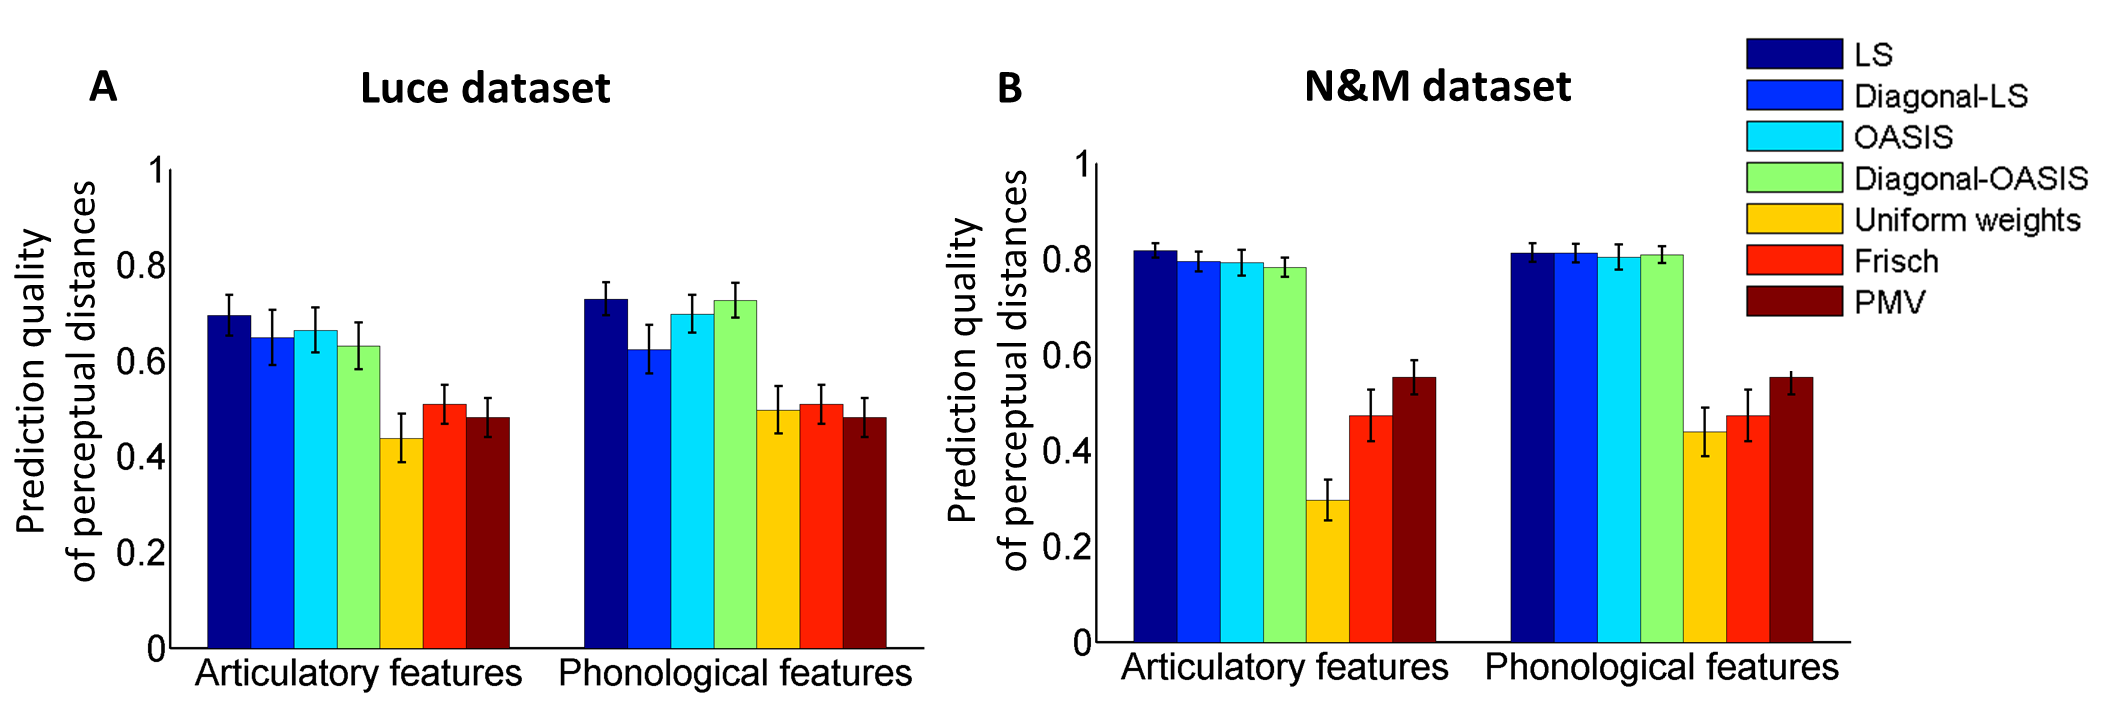
\includegraphics[width=\textwidth]{Figures/Ch2/method_comparison.png}}
\caption{Prediction quality of perceptual distances. For each of the seven methods, the Spearman correlation between the predicted and empirical perceptual distances is calculated, averaged across left-out sets. Error bars represent SD across left-out sets.} 
\end{figure}

Figure 2.2 compares the average Spearman correlation between the seven methods. Results are shown for both confusion datasets: N\&M dataset, Luce dataset; and for the two feature theories discussed above: articulatory features and phonological features. Model prediction is evaluated in a cross-validation procedure (methods 2.2.5). The prediction of the model is defined as the average Spearman correlation across all validation sets, and the standard deviation is evaluated from the distributions across these sets. To determine the optimal regularizer size model predictions are evaluated on a validation set for various values of the regularization.

Results show that learning feature weights from data significantly improves prediction in comparison to baseline methods (For the N\&M dataset, all comparisons between the data-driven methods and the theoretical measures (Frisch, PMV, uniform weighing) are statistically significant ($p$-value$<10^{-4}$, two-tailed t-test - table 2.3). The four metric-learning methods demonstrate similar predictive power, as tested on these datasets. We therefore select a method for further analysis based on model parsimony and running time. Adding a diagonal constraint results in a more parsimonious model due to its smaller number of free parameters. We therefore choose to use diagonal-LS for the analyses in the rest of this study.

\begin{table}[H]
    \centering
    \begin{tabular}{|c|c|c|c|c|}
        \hline
        \multicolumn{5}{|c|}{Luce - Articulatory features}\\
        \hline
         & LS & Diagonal-LS & OASIS & Diagonal-OASIS \\
         \hline
         Uniform weights & $<10^{-4}$ & $<10^{-4}$ & $<10^{-4}$ & $<10^{-4}$ \\
         Frisch similarity & 0.008 &    0.017 &    0.016 &    0.039 \\
         PMV & 0.003 &    0.034 &    0.006 &    0.031 \\
         \hline
         \multicolumn{5}{|c|}{Luce - Phonological features}\\
         \hline
         & LS & Diagonal-LS & OASIS & Diagonal-OASIS \\
         \hline
         Uniform weights & $<10^{-4}$ &  $<10^{-4}$ & $<10^{-4}$ & $<10^{-4}$ \\
         Frisch similarity & 0.033 &    0.012 &    0.020 &    0.011 \\
         PMV & 0.013 &    0.043 &    0.007 &    0.03 \\
         \hline
         
    \end{tabular}
    \caption{P-values of t-tests for method comparison}
\end{table}


\subsection{Perceptually-discriminative features}
Given the sparsity constraint in the optimization problem (section 2.2.2.1), we interpret the weight of each subphonemic feature as its perceptually discriminative power. We thus examine the resulting weights from each dataset, to see what they reveal about the perceptually properties of the features.

Figure 2.3 shows the learned weights from the N\&M dataset for both the articulatory and phonological-features theories.

\begin{figure}
\makebox[\textwidth][c]{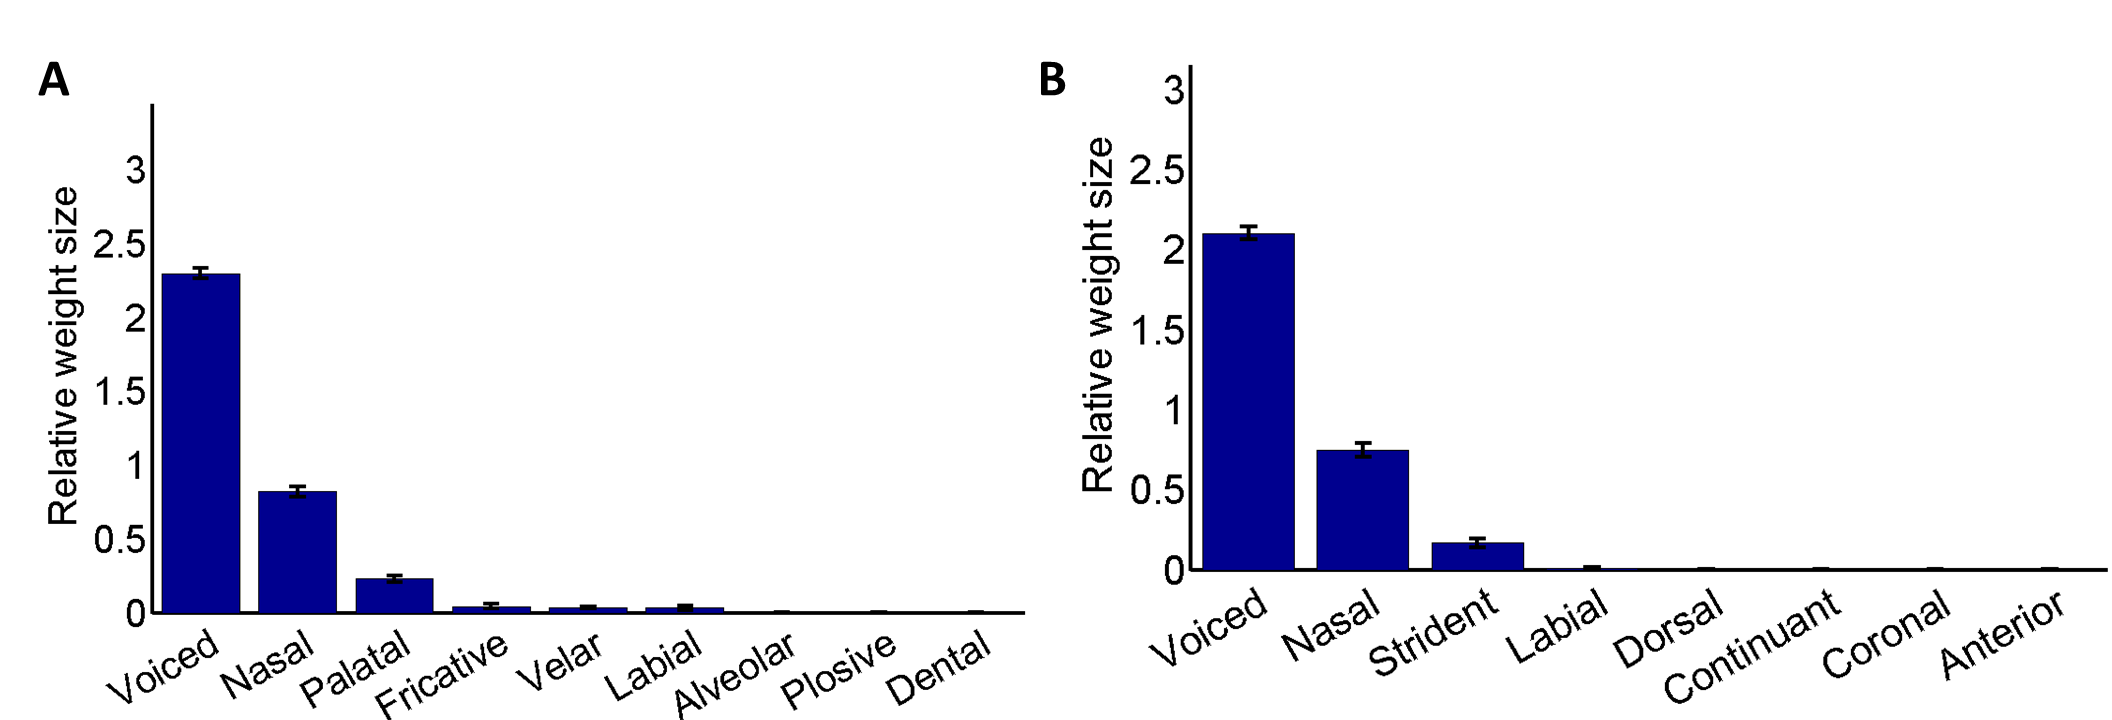
\includegraphics[width=\textwidth]{Figures/Ch2/weight_NM.PNG}}
\caption{Weights of subphonemic features as derived from the Nicely and Miller dataset. (A) Articulatory features (B) Phonological features. Error bars represent SD across validation sets.}
\end{figure}

\paragraph{Articulatory features} Among the articulatory features, the voicing feature has the highest weight, followed by the nasality feature and then the palatal one. All differences are statistically significant ($p$-value$<10^{-4}$). Next in order are the fricative, velar and labial features, which are statistically comparable. Finally, the alveolar, plosive, and dental features have weights close to zero. Note that similarly to the conclusions from the N\&M study (section 2.3.1), the voicing and nasality features in English are less affected by random noise compared to place features, and other manner features.

\paragraph{Phonological features} When ordered by their weights, the phonological features are: voicing, nasality and the strident feature, in descending order (pairwise differences are statistically significant; t-test $p$-value$<0.05$). The other features, labial, dorsal, continuant, coronal and anterior have weights close to zero. 

Comparing the results of both feature theories, voicing has the highest weight in both cases, which is then consistently followed by nasality. In the third place are the palatal feature for the articulatory theory, and the strident feature for the phonological features theory. Examining this result, we note that the only palatal phonemes in the N\&M dataset are /\textipa{S}/ and /\textipa{Z}/, both are strident consonants. Similarly, when looking into the phonemes that share the strident feature, we find that /\textipa{S}/ and /\textipa{Z}/ are again the only strident phonemes in the N\&M dataset. It therefore seems that a common property of /\textipa{S}/ and /\textipa{Z}/ is the cause for the high weight of these features, and as suggested, it seems that /\textipa{S}/ and /\textipa{Z}/ being stridents, and in particular distributed stridents, is responsible for the result. We therefore summarize the results from the N\&M dataset about the perceptual discrimination of the leading features in the following order: voicing, nasality and distributed-stridents. 

We next examine what the Luce dataset reveals about perceptual-discriminative properties of subphonemic features. Figure 2.4 presents the learned weights from the Luce dataset for both features theories.

\begin{figure}[h]
\makebox[\textwidth][c]{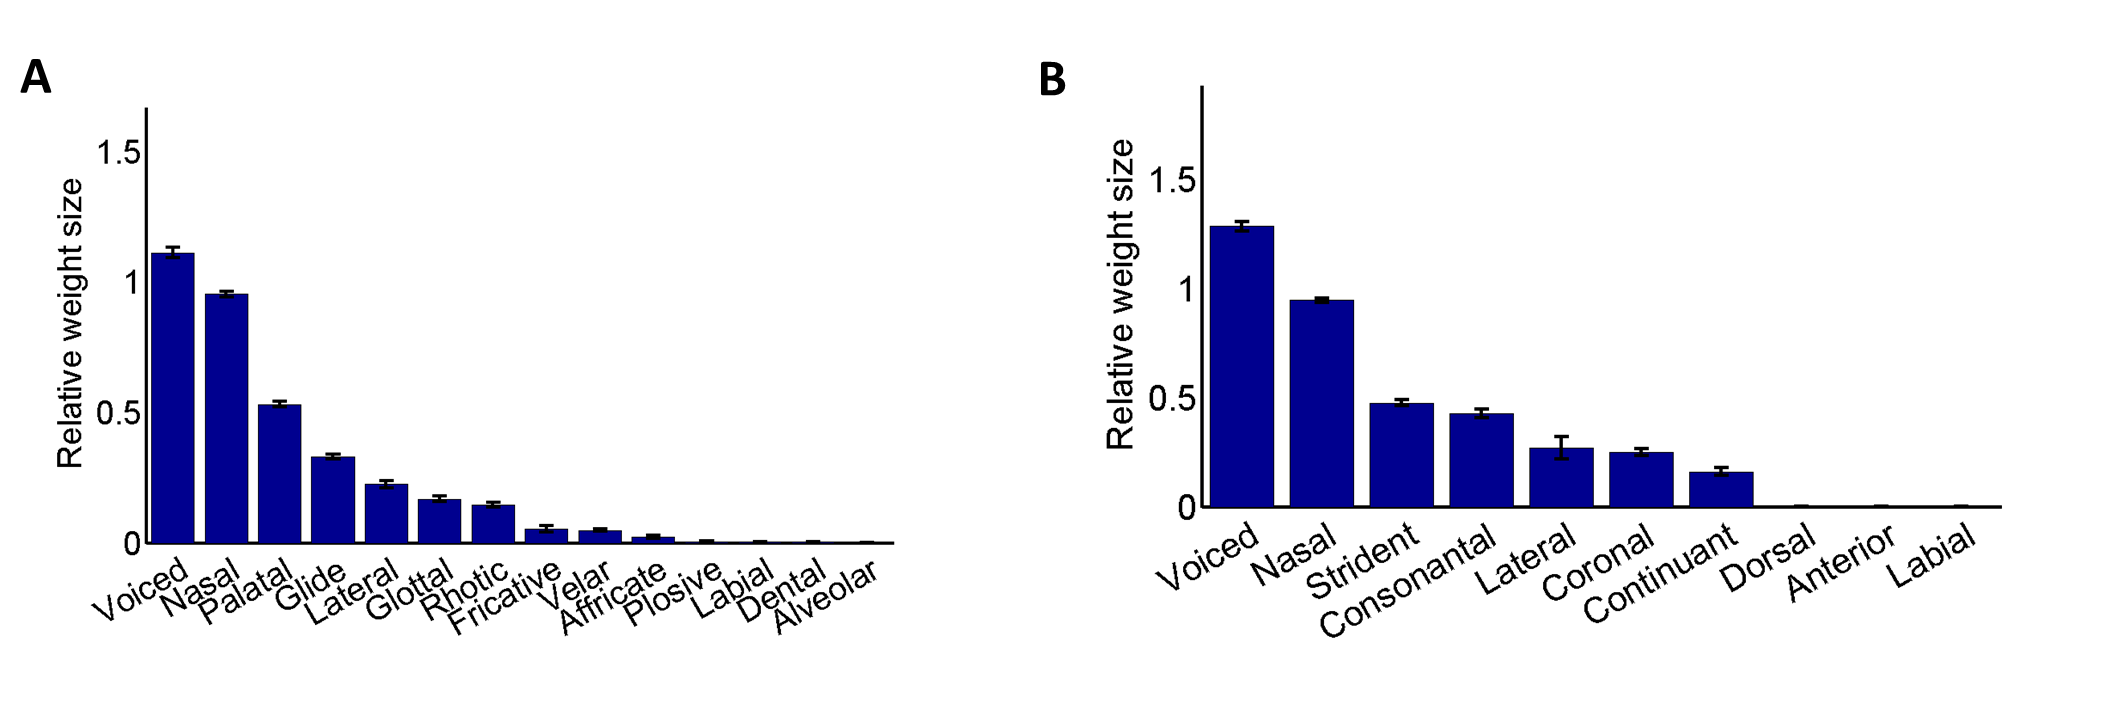
\includegraphics[width=\textwidth]{Figures/Ch2/weight_Luce.PNG}}
\caption{Weights of subphonemic features as derived from the Luce dataset. (A) Articulatory features (B) Phonological features (B). Error bars represent SD across validation sets.}
\end{figure}

\paragraph{Articulatory features} For the binary representation of articulatory features, the voicing feature has highest weight, followed by nasality, palatal, glide, lateral, glottal and rhotic features, in descending order. All differences are statistically significant (t-test $p$-value$<10^{-4}$) except for the glottal-lateral and glottal-rhotic differences. Next in order are the fricative and velar, which are statistically comparable. The rest of the features - affricate, plosive, labial, dental and alveolar features - have close to zero weights. Similarly to the N\&M dataset, the palatal feature is shared by: /\textipa{S}/, /\textipa{tS}/, and /\textipa{dZ}/, which are all distributed-strident consonants, and also by /\textipa{j}/. As for the glide, lateral, and rhotic features, the corresponding consonant phonemes are /\textipa{w}/ and /\textipa{j}/ (glide phonemes) and /\textipa{l}/ and /\textipa{r}/ (liquid phonemes). These four phonemes are characterized as approximant consonants, as the articulators are closer to each other than for vowels, without creating turbulence in the airflow as is the case with fricative consonants. 

\paragraph{Phonological features} For the phonological features, the resulting order of the subphonemic features is: voicing, nasality, strident, consonantal, lateral, coronal and continuant. All differences are statistically significant (t-test $p$-value$<0.05$) except for the lateral-coronal difference. The other features - dorsal, anterior and labial - have weights close to zero. This order follows a similar pattern to the one described so far: voicing, nasality, distributed-stridents and approximants. The two leading features are again voicing and nasality. The stridency feature, and the consonantal and lateral features, which contrast between the approximant phonemes /j/, /w/ and /l/ to other phonemes, all have relatively high weights also in this case. We therefore summarize the order between subphonemic features, based on all the results so far, as: voicing, nasality, distributed-stridents and approximants. As for the coronal and continuant features, note that they are partially redundant with respect to the leading ones and do not clearly contrast among phoneme sets. For example, the coronal feature is shared by both strident phonemes (/\textipa{s}/, /\textipa{z}/, /\textipa{S}/, /\textipa{tS}/, /\textipa{dZ}/), approximants (/\textipa{l}/, /\textipa{r}/, /\textipa{j}/) and nasal (/\textipa{n}/) phonemes, but also by /\textipa{t}/, /\textipa{d}/, /\textipa{T}/, /\textipa{D}/.

\paragraph{A two-dimensional visualization of perceived distances} To visualize the high-dimensional structure of the perceived distances in the datasets, and the relations between subphonemic features, we use Multi-Dimensional Scaling (MDS) \citep{kruskal1964}, which embeds all perceived distances on the plane. This allows us to qualitatively assess if the learned feature weights are indeed reflected in the visualization of the perceptual distances.

\begin{figure}
\makebox[\textwidth][c]{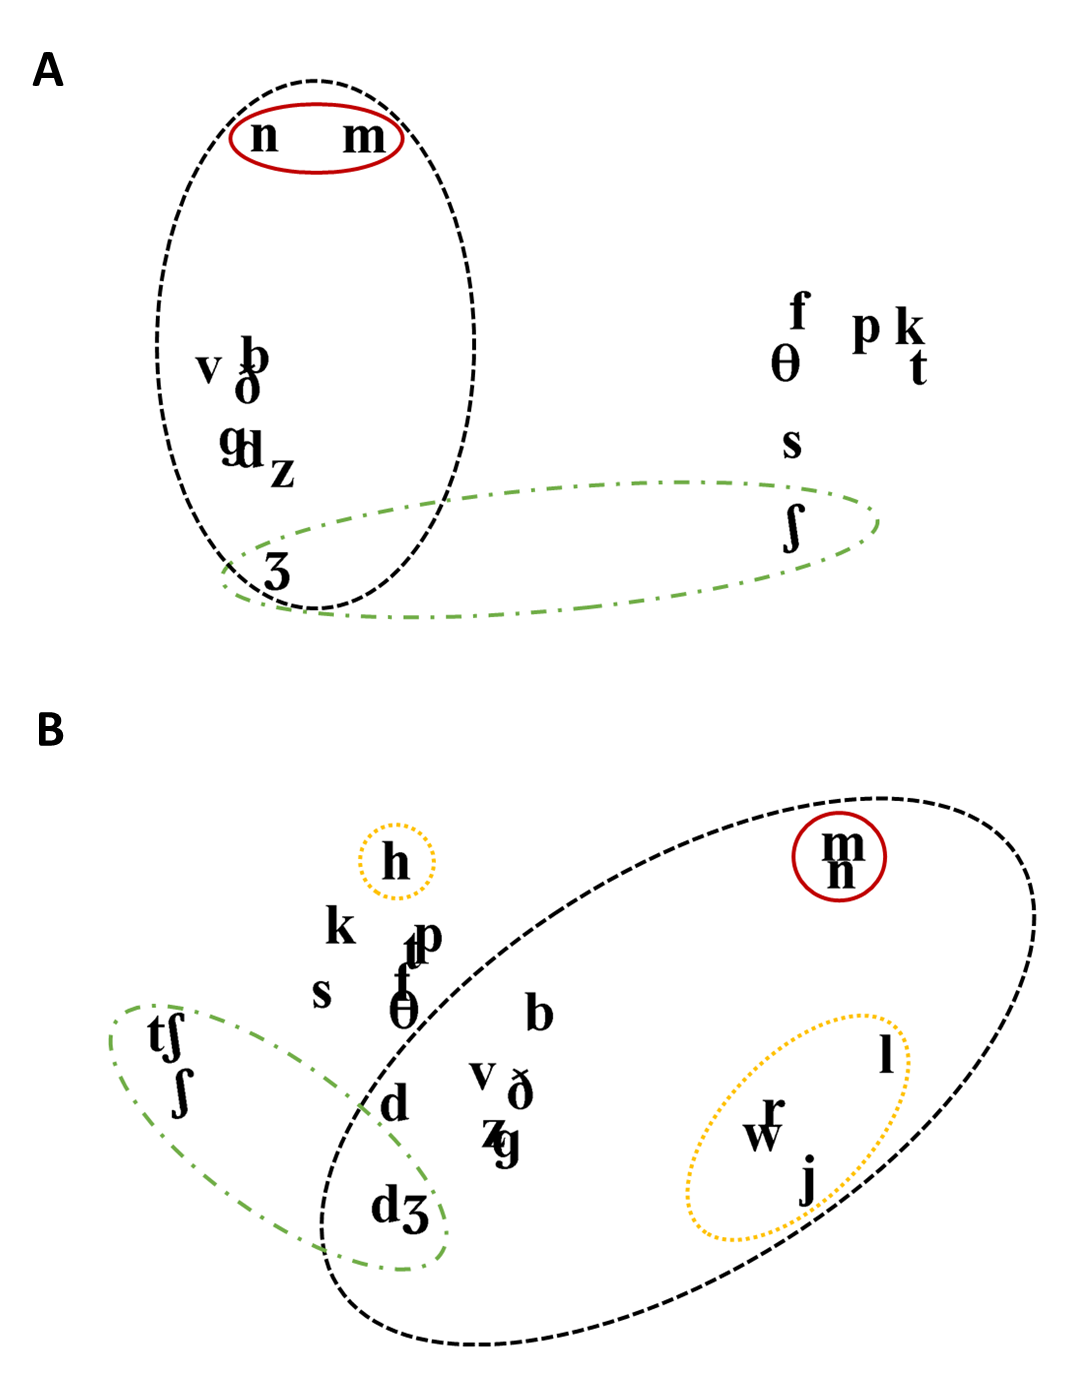
\includegraphics[width=\textwidth]{Figures/Ch2/MDS_english.png}}
\caption{Multi-Dimensional Scaling of perceptual distances between phonemes for the  (A) N\&M datset (B) Luce dataset. Ovals: black (dashed line) - voiced phonemes, red (solid line) - nasals, green - distributed stridents (dash-dot line), yellow (dotted line)- approximants}.
\end{figure}

MDS is a method for embedding objects and their pairwise distances onto a lower-dimensional space, where the distances between the objects in the lower-dimensional plane approximate the original distances. MDS was already used to explore the N\&M and other phoneme-confusion dataset \citep{Shepard1980, mielke2008emergence, Buchsbaum2015}, we test it also for the Luce dataset. Figure 2.5 presents the results of embedding the perceptual distances between all phonemes into a 2D-plane for the N\&M dataset (panel A) and for the Luce dataset (panel B). The classes of the resulting four leading features are marked with colored ovals: voiced phonemes with black (dashed line), nasal phonemes with red (solid line), distributed-strident phonemes with green (dash-dot line), and approximant-consonants with yellow (dotted line) - the last is only for the Luce dataset, as there were no approximant phonemes in the N\&M experiment. 

The MDS analysis provides several insights. First, for both datasets, voiced and voiceless phonemes reside at opposite sides of the plane. Second, nasal, distributed-strident and approximant phonemes are in the periphery of the plot, and are relatively distant from other phonemes. A phoneme will tend to result in the periphery when it is relatively distant from all other phonemes, which should match a high weight of the corresponding features. Finally, a clear distinction between distributed and non-distributed stridents is observed for both datasets. Among all stridents only the distributed stridents - (/\textipa{S}/, /\textipa{Z}/) in the N\&M dataset, and (/\textipa{tS}/, /\textipa{dZ}/ and /\textipa{S}/) in the Luce dataset - are in the periphery of the plot, whereas the non-distributed stridents (/\textit{s}/, /\textipa{z}/) are more central. This corresponds to the relatively high weights of the palatal feature that is shared by the distributed stridents but not by the non-distributed stridents. To test the variability of the MDS results, we repeated the MDS analysis leaving-out a different phoneme each time - results are qualitatively similar (not shown here).

\paragraph{Redundancy between features} To further examine the resulting feature weights, we tested how omitting a feature from the feature theory would influence the predictive power of the model and the resulting order between subphonemic features. We hypothesized that leaving out features that have relatively high weights would reduce the predictive power of the model and would affect the resulting order.

We therefore repeated the above analyses, leaving out a different feature from the representation scheme on each step, and finally estimating the new prediction of the reduced model. We present results for the larger dataset, the Luce dataset: Figure 2.6 presents the differences between the prediction of the full model and the reduced model, in ascending order of size, for each of the left-out features from the representation scheme. The prediction difference is shown for the two feature theories: articulatory features (panel A) and phonological features (panel B). The prediction difference is significant between the voicing and nasality features compared to all other features (t-test $p$-value$<0.05$), whereas results for the voicing and nasality features are statistically comparable. The palatal feature is statistically comparable to the approximant features - glide, lateral and rhotic features - and to the glottal and fricative features, and significantly different compared to the rest of the features.

\begin{figure}[h]
\vspace{.3in}
\makebox[\textwidth][c]{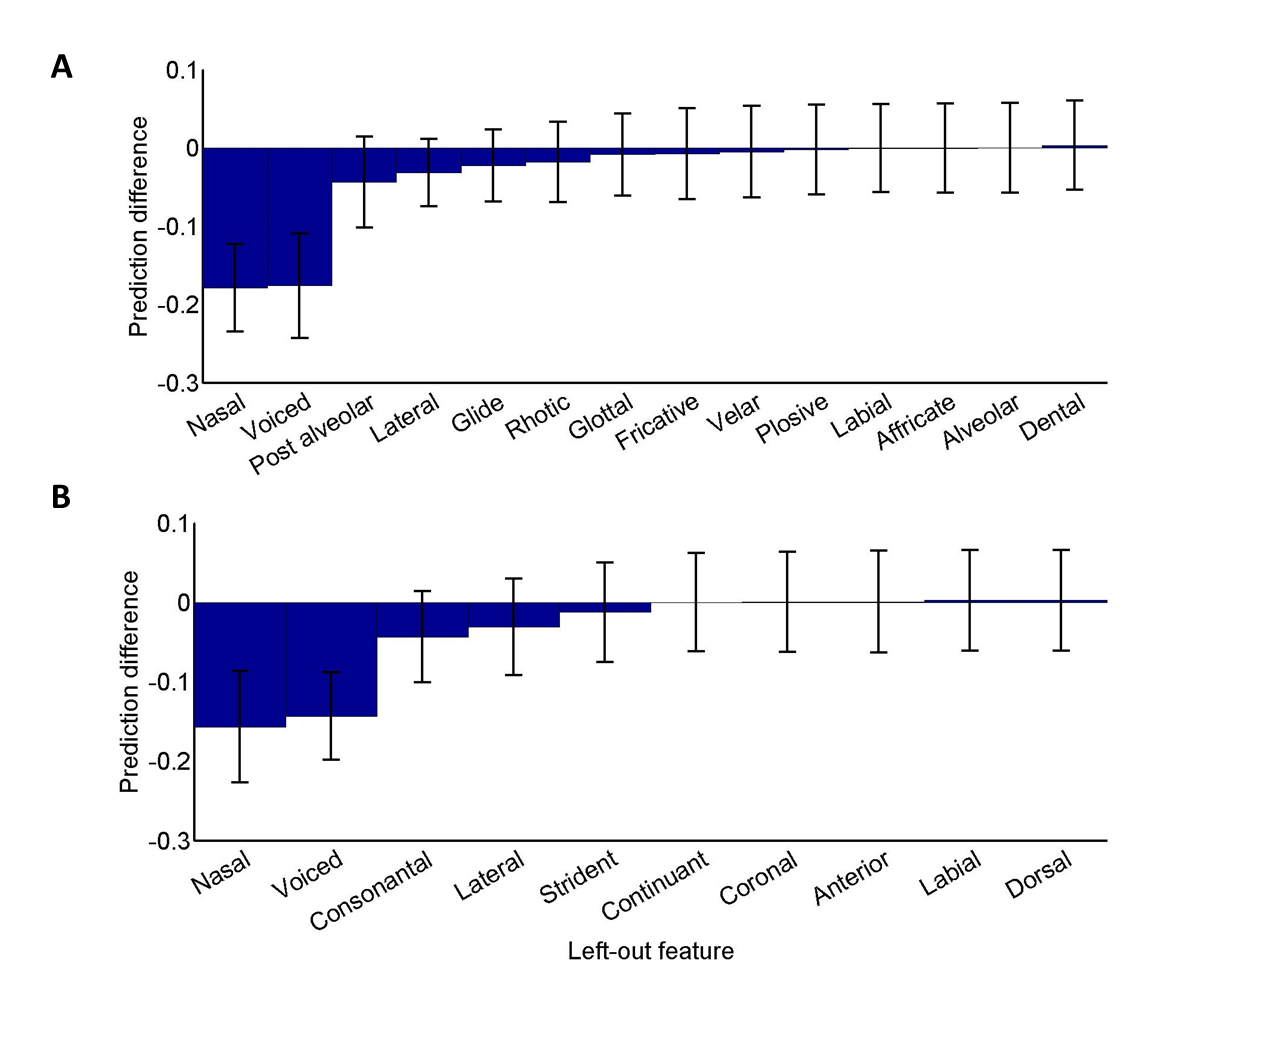
\includegraphics[width=\textwidth]{Figures/Ch2/SWR_prediction.PNG}}
\caption{Reduction in model prediction as a result of omitting a single feature, as calculated for the Luce dataset. (A) Articulatory features (B) Phonological features.}
\end{figure}

Results show that omitting high-weight features significantly reduces the predictive power of the model. In contrast, omitting low-weight features hardly affects prediction.

\subsection{Phoneme confusion in Hebrew and English}
This section analyzes the confusion data of Hebrew in the same way as for English in section 2.4.2. Hebrew phonemes are represented based on two feature theories as described above, and the LS-diagonal method is applied for each of these cases.

\begin{figure}[h]
\vspace{.3in}
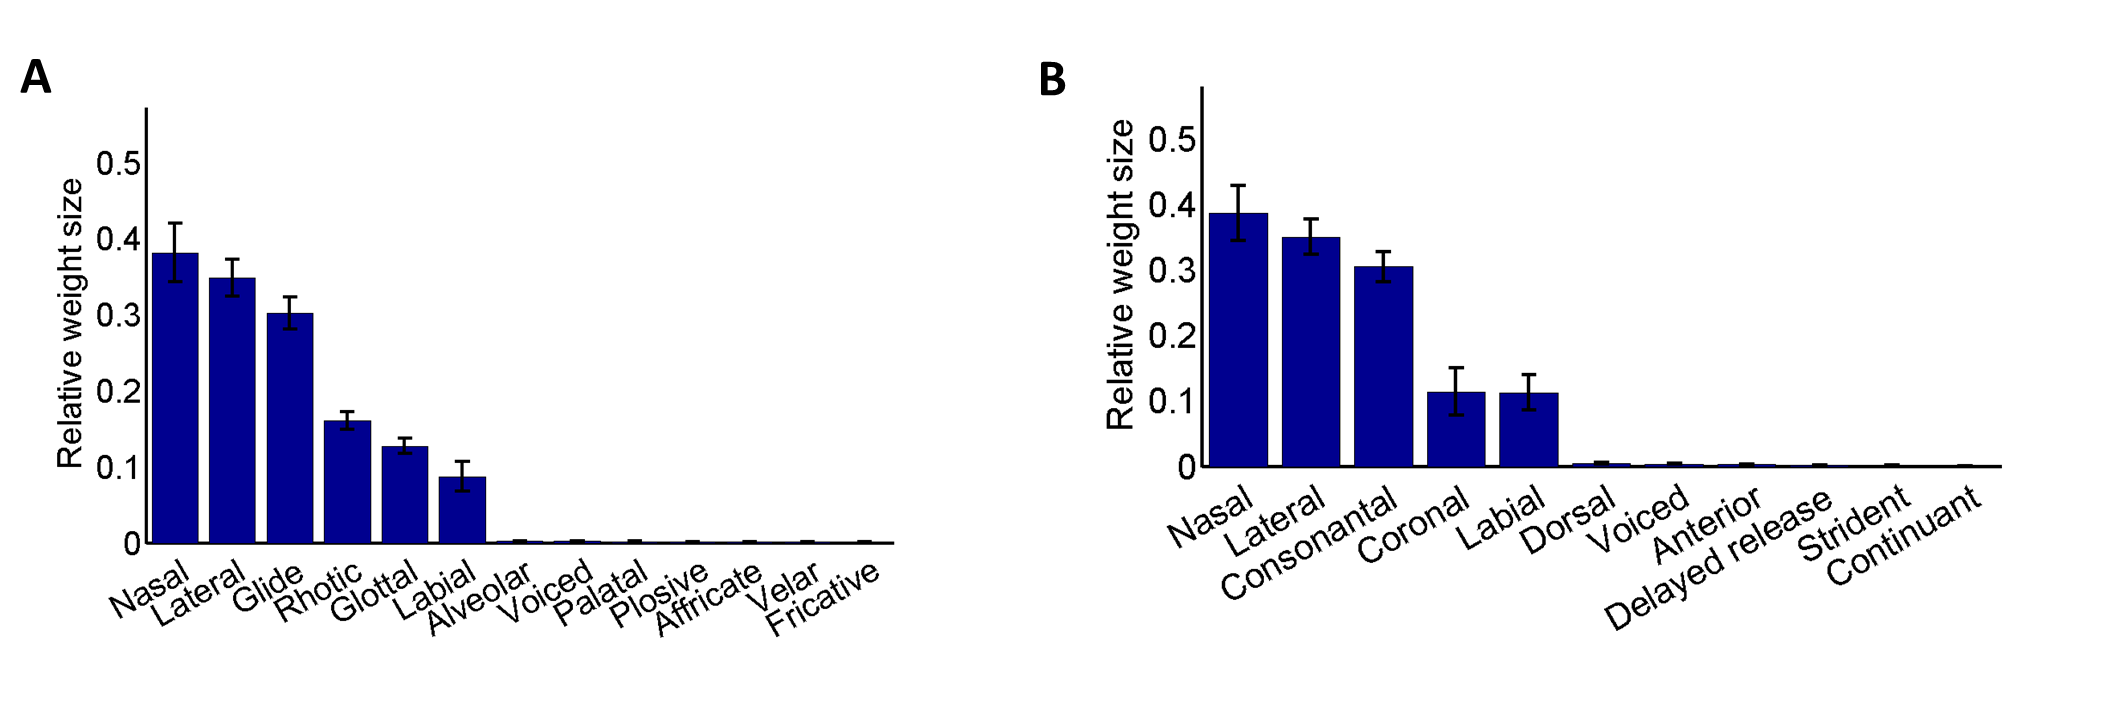
\includegraphics[width=\linewidth]{Figures/Ch2/weight_Heb.PNG}
\caption{Weights of subphonemic features as derived from the Hebrew dataset. (A) Articulatory features (B) Phonological features. Error bars represent SD across validation sets.}
\end{figure}

Figure 2.7 shows the resulting feature weights for articulatoy and phonological features. Computed for the Hebrew dataset, results show that as in English datasets, the nasality feature and the approximant features - lateral, glide and rhotic - are heavily weighted. The voicing feature, on the other hand, has much lower weight in Hebrew compared to English. In addition, the labial feature in both articulatory and phonological feature theories has relatively high weight compared to the English results.

The results of MDS analysis on the Hebrew dataset (Figure 2.8A) agree with the results of the metric learning. Nasal phonemes are embedded in the periphery of the plot, as well as the approximants and the glottal phoneme /h/. Unlike the N\&M and Luce embeddings, voiced phonemes are not well separated from unvoiced phonemes. The locations of the labial phonemes /p/ and /f/ in the MDS analysis is peripheral, which corresponds to the relatively high weight of the labial phoneme. 

\begin{figure}[H]
\vspace{.3in}
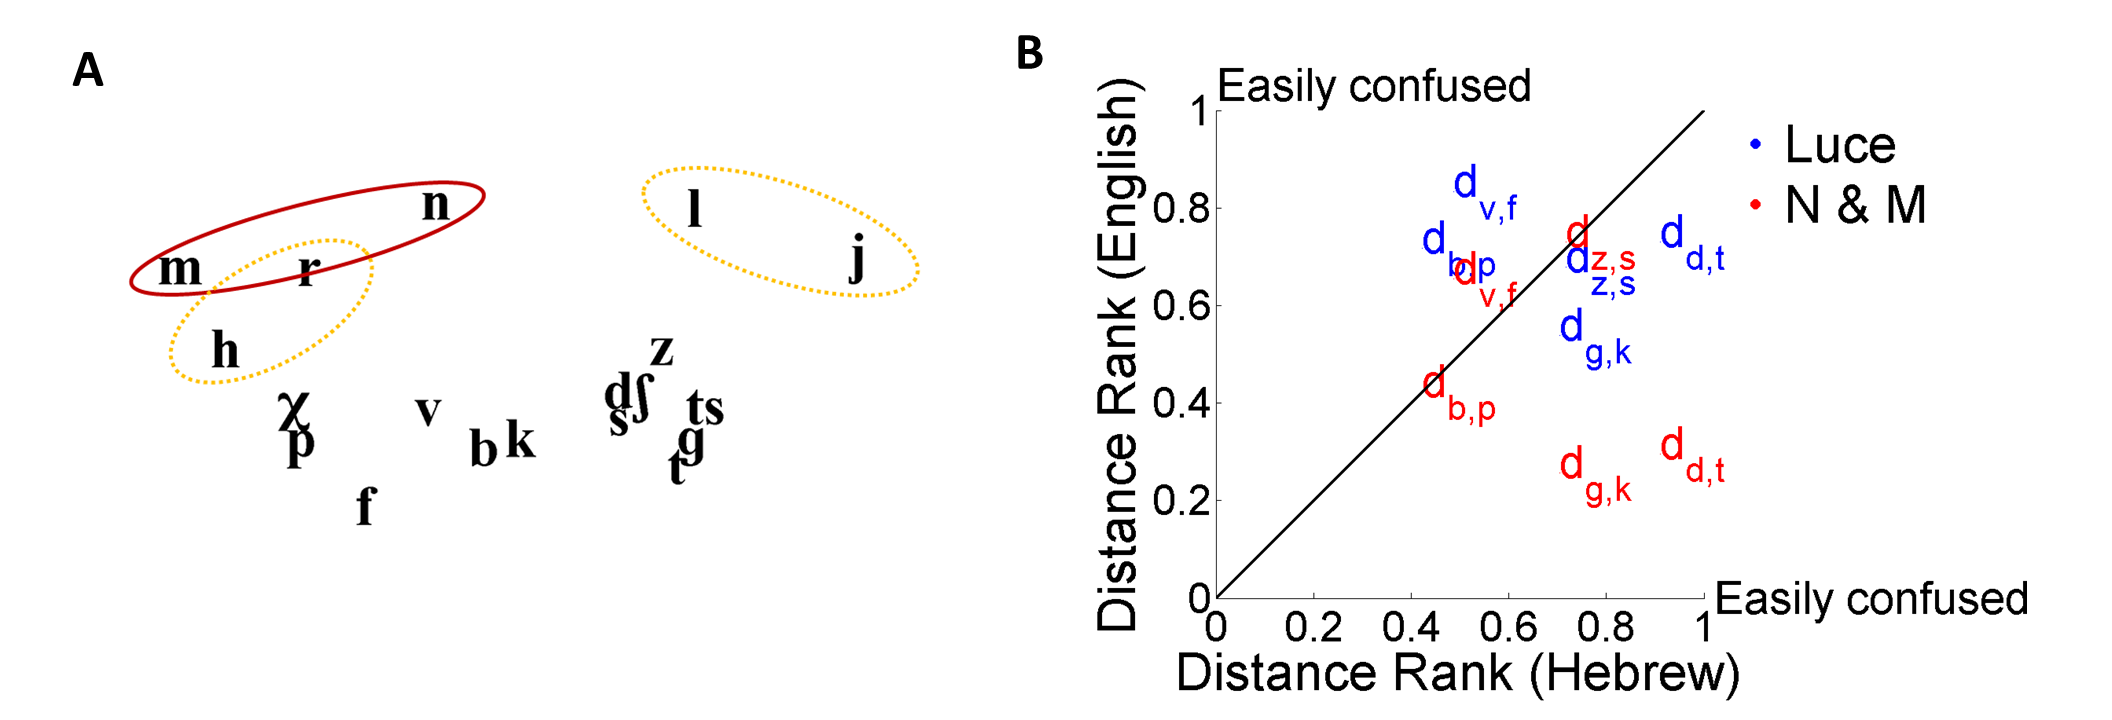
\includegraphics[width=\linewidth]{Figures/Ch2/Slide5.PNG}
\caption{(A) Multi-Dimensional Scaling for the Hebrew dataset. Ovals: red (solid line) - nasals, yellow (dotted line)- approximants and the glottal /h/(B) Voicing-differing minimal pairs: Hebrew vs. English}
\end{figure}

Figure 2.8B summarizes the differences between the Luce dataset and Hebrew with respect to perceptually-discriminative power of subphonemic features. Values on each axis represent normalized weights. Subphonmeic features that are below the line $y = x$ are more perceptually discriminative in Hebrew, and vice versa. Note that the farthest feature from the line is the voicing feature. Given this large discrepancy with respect to voicing between English and Hebrew, we further analyze this difference in the following subsection.

\subsubsection{Voicing-differing minimal pairs} To further examine the difference between Hebrew and English with respect to voicing, we compare a set of minimal pairs that only differ in voicing. We extract perceived pairwise distances between (/b/-/p/, /d/-/t/, /g/-/k/, /z/-/s/ and /v/-/f/) from the three datasets, and compare their rank on a scatter plot (figure 2.9). Ranking is necessary to equalize the distributions across languages: the values on the axes represent the rank of the perceived distance of a pair among all other pairwise distances. Before ranking distances, the largest subset of phonemes shared by all three datasets (13 phonemes) was first extracted. This was done to ensure that the rank of the distance does not depend on the specific phoneme inventory of the dataset. Features that corresponds to points above the line $y=x$ are more confusable in Hebrew than in English, and vice versa. The distance of a point from this line can serve as a measure of the difference between the two languages, with respect to the voicing difference between the phonemes in the minimal pair.

There are ten pairwise distances, five for the contrast between Hebrew and the Luce dataset (blue), and five for the contrast between Hebrew and the N\&M dataset (red). Among the ten points, five points are below the dividing line, three points above, and two reside on the line. There is a bias towards more confusion in Hebrew compared to English, with respect to voiced/voiceless phoneme confusion. This agrees with the relatively low weight of voicing in Hebrew. However, looking at the distribution of distances from the dividing line, this bias is not statistically significant (Wilcoxon rank test $p$-value$=0.57$). A possible confounding for this is the relatively high weight of the labial feature in Hebrew, in particular, the relatively large distance of /p/ and /f/ from other phonemes as can be observed in the MDS analysis. This could counteract the difference between English and Hebrew with respect to voicing. Looking at the distribution of the non-labial phonemes (/d/-/t/, /g/-/k/ and /s/-/z/) the bias towards Hebrew is significant (Wilcoxon rank test $p$-value$<0.05$).

\begin{figure} [H]
\vspace{.3in}
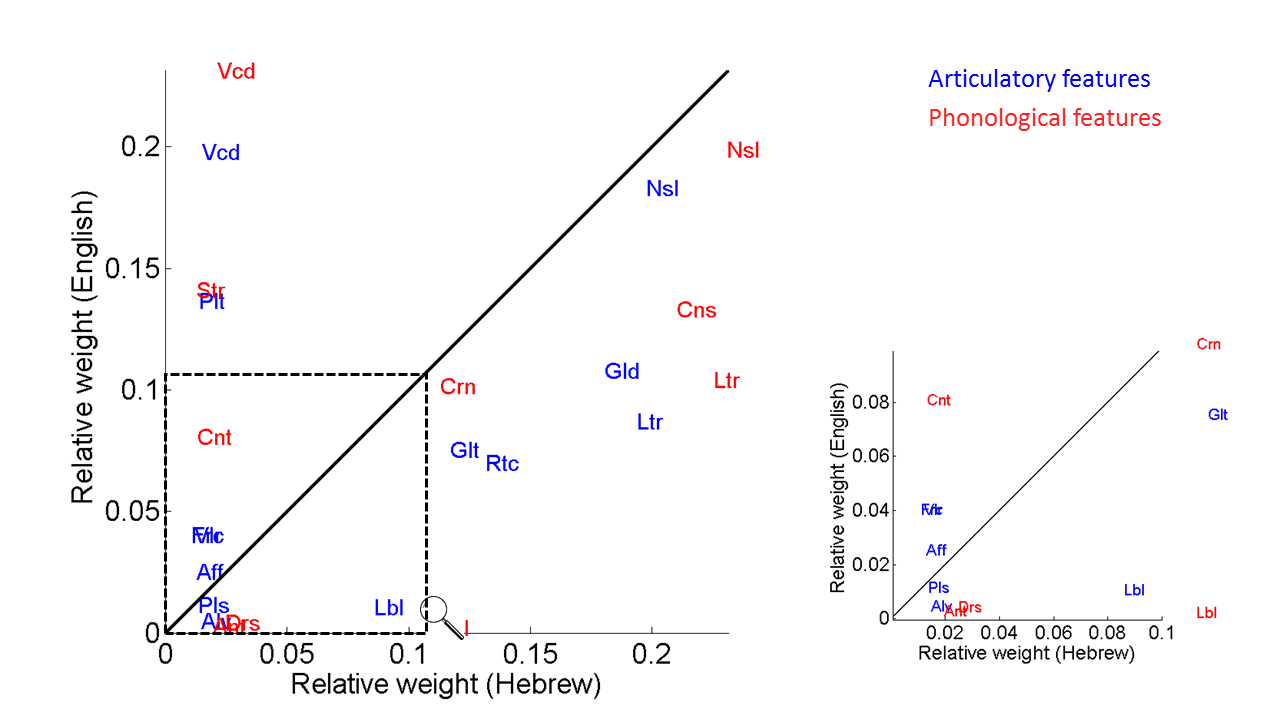
\includegraphics[width=\linewidth]{Figures/Ch2/compare_Heb_Luce.PNG}
\caption{English vs. Hebrew: relative weights of features. Articulatory features in blue, Phonological features in red. Dashed square indicates the magnified area (bottom-right). Features that corresponds to points above the line $y=x$ are more confusable in Hebrew than in English, and vice versa. Feature names are abbreviated according to their three first consonants in their name.}
\end{figure}